% Preamble
% ---
\documentclass{article}

% Packages
% ---
\usepackage{amsmath} % Advanced math typesetting
\usepackage[utf8]{inputenc} % Unicode support (Umlauts etc.)
\usepackage[ngerman]{babel} % Change hyphenation rules
\usepackage[autostyle]{csquotes}
\usepackage{hyperref} % Add a link to your document
\usepackage{graphicx} % Add pictures to your document
\usepackage{listings} % Source code formatting and highlighting
\usepackage{fancyhdr}
\usepackage{biblatex}

\author{Clemens Dautermann}
\title{Grundbegriffe des maschinellen Lernens} 
\date{\today{}}
\pagestyle{fancy}


\begin{document}
\maketitle{}
\newpage
\tableofcontents{}
\newpage

\section{Was ist maschinelles Lernen?}
Die wohl bekannteste und am häufigsten zitierte Definiton maschinellen Lernens stammt von Arthur Samuel aus dem Jahr 1959. Er war Pionier auf diesem Gebiet und rief den Begriff des \glqq machine learnings'' ins Leben. So sagte er:
\begin{quote}
	[Machine learning is the] field of study that gives computers the ability to learn without being explicitly programmed\cite{1}.
	\begin{flushright}
		---Arthur Samuel, 1959
	\end{flushright}
\end{quote}
Beim maschinellen lernen werden Computer also nicht mit einem bestimmten Algorythmus programmiert um eine Aufgabe zu lösen, sondern lernen eigenständig diese Aufgabe zu bewältigen. Dies geschieht zumeist, indem das Programm aus einer großen, bereits \glqq gelabelten'', Datenmenge mit Hilfe bestimmter Methoden, die im Folgenden weiter erläutert werden sollen, lernt, gewisse Muster abzuleiten um eine ähnliche Datenmenge selber \glqq labeln'' zu können. Als Label bezeichent man in diesem Fall die gewünschte Ausgabe des Programmes. Dies kann beispielsweise eine Klassifikation sein. Soll das Programm etwa handgeschriebene Ziffern erkennen können, so bezeichnet man das (bearbeitete) Bild der Ziffer als \glqq Input Verctor'' und die Information welche Ziffer der Copmputer hätte erkennen sollen, als \glqq Label ''. Soll jedoch maschinell erlernt werden, ein simuliertes Auto zu fahren, so bestünde der Input Vector aus Sensorinformationen und das Label würde aussagen, in welche Richtung das Lenkrad hätte gedreht werden sollen, wie viel Gas das Programm hätte geben sollen oder andere Steuerungsinformationen. Der Input Vector ist also immer die Eingabe, die der Computer erhält um daraus zu lernen und das Label ist die richtige Antwort, die vom Programm erwartet wurde. Für maschinelles Lernen wird also vor allem eins benötigt: Ein enormer Datensatz, der bereits gelabelt wurde, damit das Programm daraus lernen kann.\newline
Natürlich werden für maschinelles Lernen trotzdem Algorythmen benötigt. Diese Algorythmen sind jedoch keine problemspezifischen Algorythmen, sondern Algorythmen für maschinelles Lernen. Eine der populärsten Methoden des maschinellen Lernens ist das sogenannte \glqq Neuronale Netz''. 

\section{Neuronale Netze}
bei Neuronalen Netzen handelt es sich um eine programminterne Struktur, die für das maschinelle Lernen genutzt wird. Wie der Name bereits vermuten lässt, ist diese Methode ein Versuch das menschliche Lernen nachzuahmen.
\subsection{Maschinelles Lernen und menschliches Lernen}
Das menschliche Gehirn ist aus sogenannten \glqq Neuronen'' aufgebaut. Ein Neuron ist eine Nervenzelle, die elektrische oder chemische Impulse annimmt, und gegebenenfalls einen elektrischen oder chemischen Impuls weitergibt. Die Nervenzellen berühren sich nicht direkt sondern sind nur über die sogenannten Synnapsen verbunden, über die diese Signale übertragen werden, sodass sich ein hoch komplexes Netzwerk von milliarden von Neuronen ergibt.\footnote{
Diese Definition ist stark vereinfacht. Sie enthält ausschließlich die wesentlichen Komponenten um das menschliche Gehirn mit einem neuronalen Netz vergleichen zu können.}
\begin{figure}[h]
	\centering
	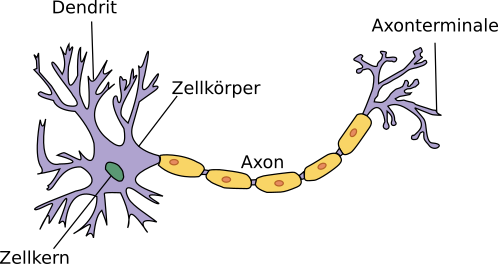
\includegraphics[]{../graphics/Neuron.png}
	\caption[Neuron \newline 
	Quelle: simple.wikipedia.org/wiki/File:Neuron.svg\newline
	Copyright: CC Attribution-Share Alike von Nutzer Dhp1080,\newline
 	bearbeitet]{Ein Neuron wie es im Gehirn vorliegt}
\end{figure}
Ein neuronales Netz ist ähnlich aufgebaut. Es besteht aus \glqq Neuronen'', die eine theoretisch beliebige Anzahl von Eingaben annehmen können und mit einer entsprechenden Ausgabe reagieren, sowie Verbindungen zwischen den Neuronen. Auch das Lernprinzip entspricht dem eines Menschen. Das Netz nimmt immer Zahlen zwischen 0 und 1 als Eingabe an und berechnet eine entsprechende Ausgabe. Es erhält anschließend die Information, wie die richtige Lösung gelautet hätte und lernt dann aus seinen Fehlern, indem es gewisse Werte, die in die Berechnung einfließen, anpasst. Analog lernt ein Mensch, indem er ausprobiert, gegebenenfalls scheitert, anschließend die richtige Antwort durch eine externe Quelle erhält und somit aus seinem Fehler lernt. Im Menschlichen Gehirn verknüpfen sich Dabei oft genutzte neuronale Verbindungen stärker und weniger benutzte Verbindungen bauen sich ab\cite{2}. Die Verstärkung und der Abbau entsprechen dem Ändern der Gewichtung einer Verbindung im neuronalen Netz. Die Gewichtung ist eine Eigenschaft der Verbindung, die eine zentrale Rolle in der Berechnung spielt und soll im folgenden weiter erläutert werden. Diese Ähnlichkeiten sind kein Zufall, sondern viel mehr Intention. Ein neuronales Netz ist nämlich der gezielte Versuch das menschliche Lernen nachzuahmen um maschinelles Lernen zu ermöglichen.
\subsection{Der Aufbau eines neuronalen Netzes}
Ein neuronales Netz besteht aus Neuronen und Verbindungen zwischen diesen. Es gibt einen sogenannten \glqq Input Layer'', der die Daten annimmt, eine beliebige Anzahl von sogenannten \glqq Hidden Layers'', in denen das eigentliche Lernen statt findet, und einen sogenannten \glqq Output Layar'', der für die Datenausgabe verantwortlich ist. Die Anzahl der Neuronen ist nach oben nicht begrenzt, wird jedoch zumeist der Aufgabe angepasst. Im Input Layer ist meißt ein Neuron pro Pixel des Eingabebildes vorhanden und im Output Layer ein Neuron pro möglicher Ausgabe. Sollen also 28$\times$28 Pixel große Bilder handgeschriebener Ziffern klassifiziert werden, so gibt es 784 Eingabeneuronen, da jedes Bild 784 Pixel groß ist, und 10 Ausgabeneuronen, da es 10 Ziffern gibt.
\begin{figure}[h]
\centering
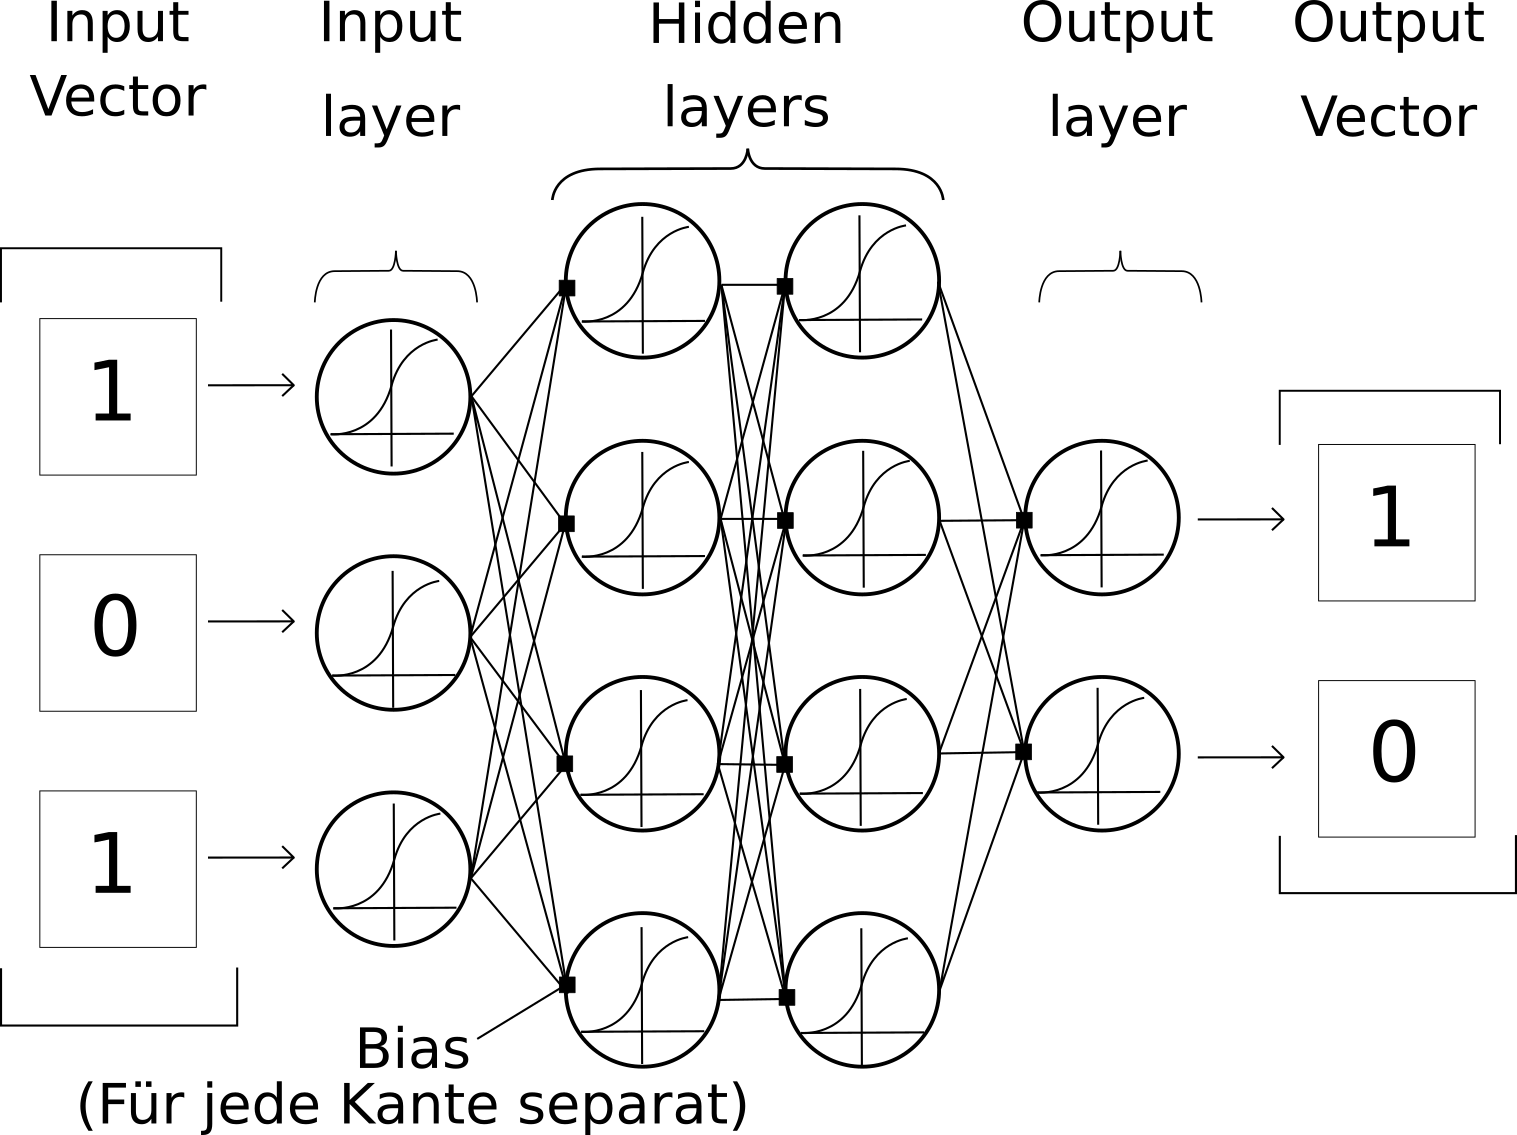
\includegraphics[width=\linewidth]{../graphics/Neural_Net.png}
\caption{Ein einfaches neuronales Netz}
\end{figure}
Jedes Neuron hat außerdem eine sogenannte Aktivierungsfunktion, die sich von Neuron zu Neuron unterscheiden kann, und jede Kante einen asoziierten Bias. Ein neuronales Netz besteht also aus:\newline
\begin{enumerate}
	\item Neuronen mit gegebenenfalls verschiedenen Aktivierungsfunktionen, aufgeteilt in ein Input-, beliebig viele Hidden- und ein Output-Layer.
	\item Verbindungen zwischen diesen Neuronen, die jeweils einen eigenen Bias besitzen.
\end{enumerate}
Sind alle Neuronen eines Layers jeweils mit allen Neuronen des nächsten Layers verbunden, wird das Layer als \glqq fully connected layer'' bezeichnet.
\newpage
\begin{thebibliography}{99}
	\bibitem{1}
	Hands-On Machine Learning with Scikit-Learn and TensorFlow\newline
	von Aurélien Géron\newline
	Veröffentlicht: March 2017 O'Reilly Media, Inc\newline
	ISBN: 9781491962282
	\bibitem{2}
	Die Logistik des Lernens eine Studie der LMU München\newline
	Quelle: www.uni-muenchen.de/forschung/news/2013/\newline f-71-13\_kiebler\_nervenzellen.html --abgerufen am 16.11.2019
\end{thebibliography}
\listoffigures
\end{document}